\documentclass[11pt]{article}
\usepackage{url}
\usepackage{algorithm}
\usepackage{algorithmic}
\usepackage{cite}
\usepackage[square, sort, numbers]{natbib}
\bibliographystyle{abbrvnat}
\usepackage[left=1in, right=1in, top=1in, bottom=1in]{geometry}
\usepackage{graphicx}

\begin{document}
	
	\title {Scheduling Algorithms}
	\author
	{    Rohith Prabakar\\
		Computer Science 351H\\
		University of Maryland\\
		UID: 115653030
	}
	\maketitle
	
	
	\section{Abstract}
	In this paper, we shall go over the problem of scheduling jobs that have no intrinsic weight.
	We shall discuss 4 different algorithms to solve the problem. The paper will go over their benefits, drawbacks, time and space complexity and when to use the algorithm. But in short, we find that the problem can be solved optimally in  $\mathcal{O}(nlogn)$ time. We will also go over other similar research paper in the literature review ({Prior Research on Related Algorithms).
		
		\section{Prior Research on Related Algorithms}
		
		\subsection{K-Bounded Preemptive Scheduling}
		
		\subsubsection{Problem Statement}
		Given a set of jobs along with their release time,  deadline, weight(higher weights are more important), number of preemptions(K) and processing time we have to find a set of jobs that can be completed such that their weights are maximized.\\
		Since we allowed preemptions (meaning that a job can be interrupted by a more important job) we have to take that into account.\\
		This Problem has been studied by Sivan Albagli-Kim, Baruch Schieber, Hadas Shachnai and Tami Tamir.
		
		\subsubsection{Input}
		
		\begin{description}
			\item[$\bullet$ line 1]  n, k - where n is the number of jobs and k is the number of preemptions
			\item[$\bullet$ lines 2 to n+1] processing time(p), release time(r), due date, weight(d) (+ve)
		\end{description}
		
		\subsubsection{Goal}
		To schedule tasks such that the weights of the jobs are maximized.
		
		\subsubsection{Why Bounded Preemption}
		For some practical tasks such as IO Scheduling, preemption is either impossible or too expensive. Thus the only good solution is to have bounded preemptive scheduling. In other words, a task can only be preempted k times.
		
		
		
		\subsubsection{Algorithmic Approximations}
		The 3 algorithms are proposed to solve the problem \citet{doi:10.1137/1.9781611974317.11}. We shall look at the algorithms and state the observations.
		\setlength{\textfloatsep}{0pt}% Remove \textfloatsep
		\begin{algorithm}
			\caption{Maximum Utilization}
			\begin{algorithmic}[1]
				\STATE Sort the jobs in non-increasing order of processing times, that is, p1 $\geq$ p2 $\geq$...$\geq$ pn.
				\STATE Consider the jobs in the sorted order
				\FOR{the current job j}
				\STATE If j can be added to the schedule, that is, if the total length of at most k + 1 idle-segments in [rj,dj) is at least pj, schedule j in the leftmost feasible way. Otherwise, reject j.
				\ENDFOR
			\end{algorithmic}
		\end{algorithm}
		\setlength{\textfloatsep}{0pt}% Remove \textfloatsep
		\begin{algorithm}
			\caption{General Greedy Scheme}
			\begin{algorithmic}[1]
				\STATE S = $\emptyset$.
				\STATE Use a certain rule to sort the jobs; consider the jobs in this order.
				\FOR{the current job j}
				\STATE If j can be added to the schedule, that is, if
				the total length of at most k + 1 idle-segments in [rj,dj) is at least pj, then schedule j in the leftmost feasible way and update S. Otherwise, reject j.
				\ENDFOR
				\STATE Return S.
			\end{algorithmic}
		\end{algorithm}
		
		\phantom{This text will be invisible}
		\begin{algorithm}
			\caption{The heuristics H\textsubscript{1} and H\textsubscript{2}}
			\begin{algorithmic}[1]
				\STATE S = $\emptyset$.
				\STATE Use a certain rule to sort the jobs; consider the jobs in this order.
				\FOR{the current job j}
				\STATE If no interval in j’s window is available, or if j was already scheduled in k + 1 segments, reject j.
				\STATE Let I be an interval with the lowest demand in j's window; schedule j in I.
				\STATE (H\textsubscript{1}) If j is not fully scheduled, and at least one of the two intervals adjacent to I is idle, schedule j on the one having minimal demand, and proceed in the same way. If both of the adjacent intervals are busy, go to step 4.\\(H\textsubscript{2}) If j is not fully scheduled, go to step 4.
				\STATE Update S and the demands on all intervals.
				\ENDFOR
				\STATE Return S.
			\end{algorithmic}
		\end{algorithm}
		\phantom{This text will be invisible}
		\subsubsection{Results}
		\begin{description}
			\item[$$ 1]  This Problem is NP hard for K = 1. This is only with unit weights. If the weights are uneven then it it's strongly np hard for k = 1. \citet{doi:10.1137/1.9781611974317.11}
			\item[$$ 2] This Problem is strongly NP hard for K $>$ 1. \citet{doi:10.1137/1.9781611974317.11}
		\end{description}
		\subsubsection{Observations}
		\begin{description}
			\item[$$ 1]  Maximum utilization algorithm uses the maximum CPU usage. We get this as we get k + 1 slots that have the maximum processing time. \citet{doi:10.1137/1.9781611974317.11}
			\item[$$ 2] General greedy scheme coincides with Maximum utilization algorithm when run on an instance of the maximum utilization problem and the jobs are considered in non-increasing order of weights.\citet{doi:10.1137/1.9781611974317.11}
			\item[$$ 3]H\textsubscript{1} and H\textsubscript{2} give higher priority to idle-intervals that are less likely to be required by other jobs. \citet{doi:10.1137/1.9781611974317.11}
			\item[$$ 4] Let density be \(\frac{np\textsubscript{max}}{2L}\) where L is the last deadline. When running all algorithms with the same inputs and different densities it is found that the performance of greedy (AlgMU) is much better than the theoretical 4-ratio. The heuristics H1 and H2 perform better than greedy for low densities and are close to each other, while for very high density, greedy performs better. \citet{doi:10.1137/1.9781611974317.11}
			\item[$$ 5]Sorting by weight is much better than sorting by the load. \citet{doi:10.1137/1.9781611974317.11}
			\item[$$ 6]The heuristics performance is mainly affected by the order in which the jobs are considered. Sorting the jobs in non-decreasing order of the ratio processing-time/weight yields the best performance. Comparing the different heuristics with the same order of jobs, the researchers conclude that the best heuristic is H2. \citet{doi:10.1137/1.9781611974317.11}
		\end{description}
		
		\subsection{Polynomial Time Algorithms for Minimizing the Weighted Number of Late Jobs on a Single Machine with Equal Processing Times}
		
		\subsubsection{Problem Statement}
		The problem is to schedule jobs such that we maximize the weights of the jobs to be completed in a given duration. In this problem, we assume that the time taken to complete each process is the same. This problem is analyzed by Philippe Baptiste.
		
		\subsubsection{Input}
		\begin{description}
			\item[$\bullet$ line 1]  n, p, d - where n is the number of jobs,  p is the processing time for each process and d is the total duration
			\item[$\bullet$ lines 2 to n+1] - w, due - where w is the weights for each process and due is when the process is due
		\end{description}
		
		\subsubsection{Goal}
		To get process p\textsubscript{1} p\textsubscript{2} ... p\textsubscript{n} such that $\sum_{1}^{n} weight (p\textsubscript{i})$ is maximum.
		
		\subsubsection{Results}
		\begin{description}
			\item[$$ 1]  When preemptions are not allowed the problem can be solved in $\mathcal{O}(n^7)$ \citet{doi:10.1002/(SICI)1099-1425(199911/12)2:6<245::AID-JOS28>3.0.CO;2-5}
			\item[$$ 2] When preemptions are allowed the problem can be solved in $\mathcal{O}(n^{4})$ \citet{DBLP:journals/corr/cs-DS-0209033}
			\item[$$ 3] Both algorithms involve dynamic programming \citet{doi:10.1002/(SICI)1099-1425(199911/12)2:6<245::AID-JOS28>3.0.CO;2-5}
			\end{description}
			
			\subsection{A Dynamic Programming Algorithm for Preemptive Scheduling of a Single Machine to Minimize the Number of late jobs}
			\subsubsection{Problem Statement}
			The problem is to schedule jobs such that we maximize the weights of the jobs to be completed in a given duration. For this problem, preemption is allowed and is not bounded by any constraint. This problem has been analyzed by E.L. Lawler in 1990.
			
			\subsubsection{Input}
			\begin{description}
				\item[$\bullet$ line 1]  n - where n is the number of jobs
				\item[$\bullet$ lines 2 to n+1] - w, due, release, p - where w is the weight for each process, due is when the process is due, release is the release date prior to which the job cannot be processed and p is the processing time.
			\end{description}
			
			\subsubsection{Goal}
			To get process p\textsubscript{1} p\textsubscript{2} ... p\textsubscript{n} such that $\sum_{1}^{n} weight (p\textsubscript{i})$ is maximum in a given time.
			
			\subsubsection{Results}
			\begin{description}
				\item[$$ 1] The time complexity of the algorithm is $\mathcal{O}(nk^2W)$ where W is the sum of all w and k is the number of distinct release dates. \citet{Lawler1990}
				\item[$$ 2] The space complexity of the algorithm is $\mathcal{O}(k^2W)$ where W is the sum of all w and k is the number of distinct release dates. \citet{Lawler1990}
				\item[$$ 3] For the problem in which the objective is simply to minimize the number of late jobs, the \\pseudopolynomial time bound becomes polynomial, i.e. $\mathcal{O}(n^3k^2)$ where W is the sum of all w and k is the number of distinct release dates. \citet{Lawler1990}
				\end{description}
				
				\subsubsection{Prelude to Algorithm}
				In this section, we go over some basic concepts to understand the time. This is to help better understand the algorithm provided by Lawler.
				\begin{description}
					\item[EDD (Earliest Due Date) rule]
					\begin{description} 
						\item[$\bullet$] Schedule jobs such that there is a decision point after every job is completed and when a new release date is encountered.
						\item[$\bullet$] At each point choose the job with the earliest due date. 
						\item[$\bullet$] This can be implemented by first sorting by release date and then by using a priority queue (Heap). This can be done in $\mathcal{O}({nlogn})$
					\end{description}
					\item[r(S)] = $\min \{r\textsubscript{j}\}$, $\forall$ j $\epsilon$ S
					\item[p(S)] = $\sum {p\textsubscript{j}}$, $\forall$ j $\epsilon$ S
					\item[w(S)] = $\sum {w\textsubscript{j}}$, $\forall$ j $\epsilon$ S
					\item[c(S)] = the time the last job in S is completed in an EDD schedule. 
					\item[C\textsubscript{j}(r, w)] Let r be a release date and w be an integer, $0 \leq w \leq W$. Define C\textsubscript{j}(r, w) to be minimum value of c(S) with respect to feasable sets S $\subset$ \{1, 2, ..., j\} with r(S) $\ge$ r and w(s) $\ge$ w. If there is no such feasible set S, then let C\textsubscript{j}(r, w) = $+\infty$. Accordingly, the maximum weight of a feasible set is given by the largest value of w such that C\textsubscript{n}(r\textsubscript{min}, w) is finite where r\textsubscript{min} = min\textsubscript{j} \{r\textsubscript{j}\}.
					\item[P\textsubscript{j - 1}(r, r\textsuperscript{'}, w\textsuperscript{''})] is the minimum processing done in interval [r\textsubscript{j}, r\textsuperscript{'}], with respect to feasible sets S\textsuperscript{''} $\subseteq$ \{1, 2, ..., j - 1\} with r(S") $\geq$ r, c(S\textsuperscript{"}) $\leq$ r\textsuperscript{'}, w(S\textsuperscript{"}) $\geq$ w\textsuperscript{"}. If there is no such feasible set S", then let P\textsubscript{j - 1}(r, r', w") = +$\infty$
				\end{description}
				
				\subsubsection{Algorithm}
				Here we go over algorithm(mostly just recurrence relations) provided by Lawer. \citet{Lawler1990}
				\begin{description}
					\item[1] Sort jobs by due date as d\textsubscript{1} $\leq$ d\textsubscript{2} $\leq$ ... d\textsubscript{n}
					\item[2] We get a recurrence relation \citet{Lawler1990}\\ C\textsubscript{j}(r, w) = min
					\begin{math}
					\left\{
					\begin{array}{l}
					C\textsubscript{j - 1}(r, w)\\
					max \{r\textsubscript{j}, C\textsubscript{j - 1}(r, w - w\textsubscript{j})\} + p\textsubscript{j}\\
					min \{C\textsubscript{j - 1}(r\textsuperscript{'}, w\textsuperscript{'}) + max \{0, p\textsubscript{j} - r\textsuperscript{'} + r\textsubscript{j} + P\textsubscript{j - 1}(r, r\textsuperscript{'}, w - w\textsubscript{j} - w\textsuperscript{'})\}\}
					\end{array}
					\right.
					\end{math}
					\\\textbf{Note} that the second condition is only true if the right-hand side does not exceed d\textsubscript{j}. If this isn't true we set C\textsubscript{j} = +$\infty$.
					\item[3] We get a relation for P. We have \citet{Lawler1990} \\ P\textsubscript{j - 1}(r, r', w") = 
					\begin{math}
					\left\{
					\begin{array}{l}
					C\textsubscript{j - 1}(r, w)\\
					max \{r\textsubscript{j}, C\textsubscript{j - 1}(r, w - w\textsubscript{j})\} + p\textsubscript{j}\\
					min \{C\textsubscript{j - 1}(r\textsuperscript{'}, w\textsuperscript{'}) + max \{0, p\textsubscript{j} - r\textsuperscript{'} + r\textsubscript{j} + P\textsubscript{j - 1}(r, r\textsuperscript{'}, w - w\textsubscript{j} - w\textsuperscript{'})\} 0  \leq w' \leq w''\}
					\end{array}
					\right.
					\end{math}\\
					With the initial conditions\\P\textsubscript{j - 1}(r, r', 0) = 0 for j = 1, 2, ..n.\\P\textsubscript{0}(r, r', w") = +$\infty$ for w" $>$ 0.
					\item[4] With this we can get a subset S with maximum weight.
				\end{description}
				
				\subsubsection{Complexity}
				\begin{description}
					\item[$\bullet$] Time taken to complete P\textsubscript{j - 1}(r, r', w") for each iteration is $\mathcal{O}(k^2W^2)$ \citet{Lawler1990}
					\item[$\bullet$] Time taken to complete C\textsubscript{j}(r, w) for each iteration is $\mathcal{O}(k^2W^2)$ \citet{Lawler1990}
					\item[$\bullet$] Thus the time complexity is $\mathcal{O}(nk^2W^2)$ \citet{Lawler1990}
					\item[$\bullet$] Thus space complexity is $\mathcal{O}(k^2W)$ \citet{Lawler1990}
				\end{description}
				
				\subsection{Scheduling n Jobs with Equal Release Dates}
				\subsubsection{Problem Statement}
				The problem is to n schedule jobs such that we maximize the weights of the jobs to be completed in a given duration. For this problem, we assume that all jobs have the same release time and are associated with a monotone non decreasing deferral cost function. The Well known algorithm of Moore and Hodgson solves this problem. \citet{doi:10.1287/mnsc.15.1.102}
				
				\subsubsection{Input}
				\begin{description}
					\item[$\bullet$ line 1]  n - where n is the number of jobs
					\item[$\bullet$ lines 2 to n+1] - w, d - where w is the weight for each process and due is when the process is due
				\end{description}
				
				\subsubsection{Goal}
				To get process p\textsubscript{1} p\textsubscript{2} ... p\textsubscript{n} such that $\sum_{1}^{n} weight (p\textsubscript{i})$ is maximum in a given time.
				
				\subsubsection{Result}
				\begin{description}
					\item[1] This problem can be solved in $\mathcal{O}(nlogn)$ \citet{doi:10.1287/mnsc.15.1.102}
				\end{description}
				
				\subsection{Brief Note on Preemptions}
				\label{bnop}
				\textbf{What are Preemptions?} \\Preemptions is just a fancy way of saying interruptions while running a program. If we find a proper schedule of jobs j\textsubscript{1}, j\textsubscript{2}, ...j\textsubscript{n} that maximizes weight and we get a new job j\textsubscript{k} that when included gives a different set of jobs that maximizes weight we have two options
				\begin{description}
					\item[1] We can stop running the current job and run the sequence of jobs that produce the optimum solution.
					\item[2] We can finish running the current job and then recompute the optimum solution and run those set of jobs.
				\end{description}
				The first version is an example of preemption. There are some benefits and drawbacks to preemption.\\
				The \textbf{benefits} are that it might be faster for certain types of problems.\\
				The \textbf{Drawbacks} of preemptions are that preemptions have a certain overhead which might be more expensive than just letting the program finish. Hence if the overhead is more expensive than an average program, preemptions should be avoided.
				
				\section{Problem Statement}
				The problem is to schedule jobs such that we maximize the weights of the jobs to be completed in a given duration. However, for this problem we consider all of the weights to be the same. Hence we just want the set of jobs that can be completed in a given duration such that the set has the maximum number of jobs. For this problem, there can be a constant stream of input and our algorithm must produce the best set of jobs. For this problem, we do not allow preemptions. The reasons are stated in section \ref{bnop}
				
				\subsection{Why This Problem?}
				These days there are many applications that have processes without a notion of weight(importance). If we look at WhatsApp, there is a server that receives and sends messages. It is difficult to gauge the importance of one message over another. In fact, If you wanted to do analyze the message to get an estimate of its importance, it will be a huge privacy violation of the user. Similarly, in applications such as email, youtube and even car ride services such as uber, all of the individual transactions are equally important. Hence, the performance of a service is based on the number of individual transactions that are completed.\\
				The algorithm must be able to accept streams of input to model real-world data. Person A might request a ride at 10 am and a person B can request a ride at 10:01 am. We should organize our service such that both user's request is fulfilled.
				
				\subsection{Input}
				\begin{description}
					\item[Line 1] n where n is the number of Jobs.
					\item[Line 2 to n + 1] b d p where d is the deadline and p is the processing time required and b is the start time.
				\end{description}
				\textbf{Note} For this problem, we only get the info about a job exactly on its begin time. To implement a streaming interface we will use an array of all info and only add on the to be processed list on ints begin time. For this problem, each loop iteration is a unit of time. So the first time we go through the loop one second will pass. This is to abstract all the complicated time comparisons away and get a small simplified problem to work with. For this problem, we store the input as a list. so the first index represents the begin time, second the deadline and third the processing time.
			
				
				\subsection{Goals}
				To get a set of process p\textsubscript{1} p\textsubscript{2} ... p\textsubscript{n} such that n is maximum.
				For simplicity, we shall just return n. In the following few sections, we will discuss various algorithms to solve this problem, analyze its complexity and find its tradeoff. We will then go over the ideal algorithms one should use to solve the problem.
				
				\subsection{Preprocessing}
				Before we discuss the algorithms, let's talk about how we are going to implement it.\\
				\textbf{Note} Not all algorithms require preprocessing.
				
				\begin{description}
					\item[$\bullet$] Lets store all the jobs to be processed in a list. Let us then sort it by beginning time.
					\item[$\bullet$] Lets now loop over till this list is empty. We will have another list (newlist) that stores all the jobs that we can process (begin time $<$ current time).
					\item[$\bullet$] Here We pick a job from newlist. Then we remove it from the newlist and the original list. We then increment the time as time is simplified to measure iterations. Our algorithms deal with how we pick the job to be processed from the newlist.
				\end{description}
				Some of the Code(item 1) for preprocessing is present in the main method in main.py. Others will be handled within the different algorithms.
				
				\subsection{Naive Trivial Algorithm}
				\subsubsection{Logic}
				The Easiest way to solve the problem is to permute all of the elements in the newlist. We then check each of the permutations as to how many jobs can be completed within the time.
				
				\subsubsection{Complexity}
				The Time complexity for finding all permutations is $\mathcal{O}(n!)$. The Algorithm for finding the number of jobs for each list is $\mathcal{O}(n)$. \\
				Thus overall time complexity for this algorithm is $\mathcal{O}(n*n!)$.
				Also, we need $\mathcal{O}(n!)$ space to store the permutations.
				
				\subsubsection{Algorithm}
				Let us go over the trivial algorithm
				\begin{algorithm}
					\caption{Naive Trivial Algorithm}
					\begin{algorithmic}[1] 
						\STATE allPermutations = permute(list) // Note list is the list of jobs we got
						\STATE result = 0
						\FOR{lst in allPermutations}
						\STATE maxNo = findNoComplete(lst)
						\STATE result = max(maxNo, result)
						\ENDFOR
						\STATE return result
					\end{algorithmic}
				\end{algorithm}
				
				Now let us go over the algorithm to find the number of jobs that can be accomplished (findNoComplete).\\
				Remember that this function takes a list as an argument.
				
				\subsubsection{Algorithm For Finding the number of jobs that can be Accomplished}
				\phantom{This text will be invisible}
				
				\begin{algorithm}
					\caption{findNoComplete}
					\begin{algorithmic}[1] 
						\STATE if length of list = 0 then we return 0
						\STATE time = list[0][0] // begin time of first element in list
						\STATE res = 0 // the number of jobs in list we can finish consecutively
						\FOR{lst in list}
						\STATE B, D, P = lst[0], lst[1], lst[2] // the begin time deadline and end time for the given process
						\IF{time + P $<$ D }
						\STATE // Note that here the process can be completed within the given time
						\STATE res = res + 1
						time += P
						\ENDIF
						\ENDFOR
						\STATE return res
					\end{algorithmic}
				\end{algorithm}
				
				\subsubsection{Pros and Cons of this algorithm}
				This algorithm involves very little mental effort to code. However, it takes $\mathcal{O}(n*n!)$ time which is bad. Also it takes $\mathcal{O}(n!)$ space too. We can do much better.
				
				\subsection{Implementing a Streaming Algorithm}
				In this section, we will go over how we implement the streaming algorithm.\\
				We have a timer variable that keeps track of the current time. We will go over the list (Which is sorted when preprocessed). We also have a list(toProcess) that contains all the elements that can be processed.
				
				\begin{description}
					\item[$\bullet$] First we loop over till the time $<$ the last elements begin time (which is the last begin time since its sorted) - 
					\begin{description}
						\item[1] While the first element in the lst has begin time which is in between the previous begin time and the current time and has a deadline after the current time, pop the first element and add to toProcess.
						\item[2] Find the best item that is to be processed using another algorithm. Add the processing time to time
						\item[3] Remove all elements that have a deadline before the current time.
					\end{description}
					\item[$\bullet$] Now that the toProcess list is completed, we just have to finish processing the remaining elements. So we repeat the previous step (processing and updating time). We do this until the toProcess list has no elements.
					\item[$\bullet$] We can implement the same algorithm to the trivial algorithm to make it a streaming capable algorithm.
				\end{description}
				
				\subsection{An Improved Algorithm}
				Now let us try to find a much better algorithm for the problem. With a little bit of effort, we can do much better than $\mathcal{O}(n*n!)$ time!
				
				\subsubsection{Logic}
				Instead of looking at all possibilities, a simple observation can get us very far.\\
				\textbf{Observation:} If we can complete jobs A and B within the given time, then we can \textbf{always} process them in increasing order of deadlines.\\
				This might look obvious but can help us simplify the algorithm a lot. With this, we can sort by the deadlines, and find a sequence of consecutive jobs such that they can all be completed in time. The maximum such pair is the result.
				\\ Let us now look at the algorithm
				
				
				\begin{algorithm}
					\caption{Improved Algorithm (takes input: toProcess - a list and time)}
					\begin{algorithmic}[1] 
						\STATE sort toProcess based out of deadline
						\STATE res, min = 0, 0
						\FOR{i from 0 to toProcess.length}
						\STATE cnt, t = 0, time
						\FOR{j from i to toProcess.length}
						\STATE cur = toProcess[j]
						\IF{time + cur[2] $<=$cur[1]}
						\STATE cnt += 1
						\STATE time += cur[2]
						\ELSE
						\IF{cnt $>$ min}
						\STATE min = cnt
						\STATE res = i
						\ENDIF
						\ENDIF
						\ENDFOR
						\ENDFOR
						\STATE return toProcess[res]
					\end{algorithmic}
				\end{algorithm}
				
				\textbf{Note} This makes an assumption that there will not be a task that is so much more expensive than the others. If so that algorithm won't give the best result (but will give a very close approximation). To see the problem if we have a sequence of jobs  1, 2, 3 (sorted by the deadline). If 2 is computationally very expensive then the best solution will be 1, 3. Our algorithm will not find the solution (but gives a really close result).
				
				\subsubsection{Complexity}
				If we look over the algorithm we see that we sort the list. Sorting is an $\mathcal{O}(nlogn)$ operation.
				After that, we find the best starting job. This operation takes $\mathcal{O}(n^2)$. So overall the total time complexity is $\mathcal{O}(n^2)$. We also don't use any more space than the space for storage of data, hence it is space efficient.
				
				\subsubsection{Naive vs Improved Algo}
				Lets us now compare the two mentioned algorithms. We already know the time complexity but how do they compare in a real-world test? If you look at figure 1 we see that improved algorithm is much better than the naive algorithm. However, we can do much better. Let's look for a more optimal solution.
				
				\begin{figure}
					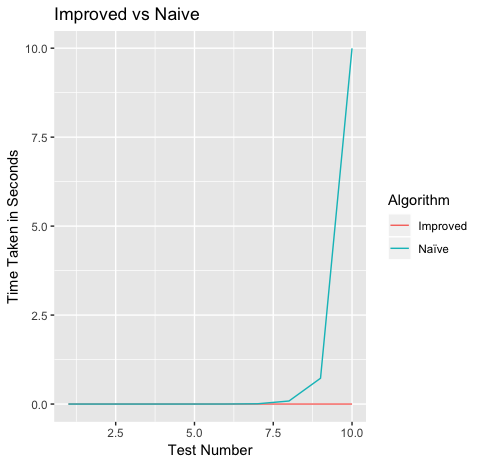
\includegraphics[scale=0.5]{ImprovedVsNaive.png}
					\caption{Improved Algo vs Naive Algo}
				\end{figure}
				
				\subsection{Optimal Algorithm}
				\subsubsection{Logic}
				Instead of going through each index and iterating over the index, we can use a sliding window approach to shorten the time. We can have a start index and end index. We can move the end pointer until we reach a point such that the tasks cannot be completed within the given time. At this point, we can move the start pointer to the right. We can look at the algorithm below.
				
				\begin{algorithm}
					\caption{Optimal Algorithm (takes input: toProcess - a list and time)}
					\begin{algorithmic}[1] 
						\STATE sort toProcess based out of deadline
						\STATE res, cnt, start, end = 0, 0, 0, 0
						\WHILE{start $<$ toProcess.length}
						\STATE count = 0
						\WHILE{end $<$ toProcess.length}
						\STATE cur = toProcess[end]
						\IF{time + cur[2] $<=$cur[1]}
						\STATE count += 1
						\STATE end += 1
						\STATE time += cur[2]
						\ELSE
						\STATE break
						\ENDIF
						\ENDWHILE
						\IF{cnt $>$ cnt}
						\STATE cnt = count
						\STATE res = start
						\ENDIF
						\STATE time -= toProcess[start][2]
						\STATE start += 1
						\ENDWHILE
						\STATE return toProcess[res]
					\end{algorithmic}
				\end{algorithm}
				
				
				\begin{figure}
					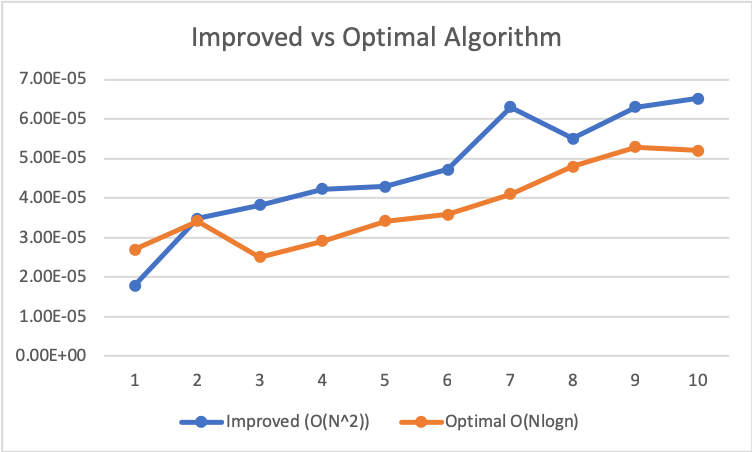
\includegraphics[scale=0.5]{ImprovedVsOptimal.png}
					\caption{Improved Algo vs Naive Algo}
				\end{figure}
				
				\subsubsection{Complexity}
				If we look over the algorithm we see that we sort the list. Sorting is an $\mathcal{O}(nlogn)$ operation.
				After that our sliding window approach takes $\mathcal{O}(n)$. So overall our time complexity is $\mathcal{O}(nlogn)$. It is much better than our Improved algorithm. We see in Figure two their real-world performance.
				
				\subsection{Other Algorithms}
				There are two other algorithms we can use to solve this problem. We will look at both below and discuss their benefits and drawbacks.
				
				\subsubsection{Greedy Algorithm 1}
				At each part of the process, we can choose to perform the job that takes the minimum processing time that can be computed. This algorithm can be done in $\mathcal{O}(n)$ time.\\
				\textbf{Benifits:} We can see that such an algorithm would lead to high efficiency. This can be done if the jobs to be processed is a lot faster than the scheduling algorithm. (We don't want the algorithm to do the scheduling take more time than the process).\\
				\textbf{Drawbacks:} It will not lead to accurate results.
				
				\subsubsection{Greedy Algorithm 2}
				At each part of the process, we can choose to perform the job that has the first deadline. This algorithm can be done in $\mathcal{O}(n)$ time. This has the same benefits and drawbacks as greedy algorithm 1. However, the difference is that we will always choose to compute the task that has to be done first. This has different use cases as Greedy Algorithm 1.
				
				\subsection{Summary}
				We have discussed different solutions to the scheduling problem with equal weights.
				We have found that
				\begin{description}
					\item[1] The Algorithm can be solved optimally in $\mathcal{O}(nlogn)$ time.
					\item[2] There are good greedy solutions that can be done in $\mathcal{O}(n)$ time that has different use cases.
				\end{description}
				\pagebreak

			\section{Appendix}
			\bibliography{References}
			\end{document}
			
			
			
			
			
			
			
			
			
			
			
			
			
			
			
			
			
			
			
			
			
			
			
			
			
			
			
			
			
